\documentclass[a4pper,11pt,onecolumn]{article}
\setlength\parindent{2em}
\usepackage{graphicx}
\usepackage{authblk}
\title{Group Practical 2 }
\author[*]{Shiyu Yi,2016141231175\\Chuang Du,2016141462277\\Jiali Shang,2016141462137}

\renewcommand\Authands{ and }
\begin{document}

\maketitle

%section
\section{Objectives:}


\begin{itemize}
	
	\item[-] To understand the application of basic clustering techniques to expression data.
	
	\item[-] To illustrate how clusters can be analysed on the basis of their statistical validity.
	
	\item[-] To illustrate how obtained clusters and validity indicators can be used to support
	biological interpretation.
\end{itemize}

\section{Activities:}

\subsection{Problem 1}

Which information is represented by columns (and rows) in the table displayed? How many samples are included? How many natural classes describe this problem?\\

Answer:

Each column represents the numerical level of a gene in a different sample

Each row represents the numerical level of different genes in each sample.

38 samples are included.

2 natural classes : AML and ALL

\subsection{Problem 2}

Examine the obtained partitions. Are samples belonging to the same classes (ALL and AML) generally clustered together? Can outliers or exceptions to this rule be identified?\\

No, they are not.When K = 2, it's basically all together. When K= 3, ALL is basically together, AML is basically not together, when K is equal to 4, ALL is basically together, and the absence of AML is strengthened.

We don't think it can be sure the outliers or exception.

\subsection{Problem 3}

According to this validity index, which is the best partition or correct number of clusters?

\begin{table}[h]  %table 里面也可以嵌套tabular,只有tabular是不能加标题的
	\centering  %表格居中
	\caption{Calculate Dunn's Index}  %表格标题
	\begin{tabular}{cc}  %右对齐
		\hline
		\hline
		k & Dunn's Index \\ [0.5ex] 
		\hline
		 2 & 1.368677784020677   \\
		 3 & 0.9617664356001026 \\
		 4 & 0.7123988365558371  \\
	
		\hline
		\hline
	\end{tabular}
\end{table}

So k=2 is the best.It match our actual situation

\subsection{Problem 4}
Repeat the same cluster validity procedure using another validity index. Compare results.\\

choose Goodman-Kruskai Index

\begin{table}[h]  %table 里面也可以嵌套tabular,只有tabular是不能加标题的
	\centering  %表格居中
	\caption{Calculate Goodman-Kruskai Index}  %表格标题
	\begin{tabular}{cc}  %右对齐
		\hline
		\hline
		k & Goodman-Kruskai Index \\ [0.5ex] 
		\hline
		2 & 0.9320598006644518   \\
		3 & 0.8861171748468418 \\
		4 & 0.7596945732206163  \\
		
		\hline
		\hline
	\end{tabular}
\end{table}

Still,k=2 is the best.

\subsection{Problem 5}

Repeat these cluster validity procedures using other intra- and inter-cluster distances. Compare results.\\

So we changed the Metrics from Euclidean to Manhattan

\begin{table}[h]  %table 里面也可以嵌套tabular,只有tabular是不能加标题的
	\centering  %表格居中
	\caption{Calculate Dunn's Index(Manhattan)}  %表格标题
	\begin{tabular}{cc}  %右对齐
		\hline
		\hline
		k & Dunn's Index \\ [0.5ex] 
		\hline
		2 & 1.9393051013997842   \\
		3 & 1.0539531093492691 \\
		4 & 0.7804016773339219  \\
		\hline
		\hline
	\end{tabular}
\end{table}

Still, k=2 is the best.It match our actual situation

\subsection{Problem 6}

Using a table aggregate these results for each number of clusters, estimate the  correct number of cluster.\\

\begin{table}[h]  %table 里面也可以嵌套tabular,只有tabular是不能加标题的
	\centering  %表格居中
	\caption{Estimate the correct number}  %表格标题
	\begin{tabular}{ccccc}  %右对齐
		\hline
		\hline
		K& AML'S Error & AML'S Correct number& ALL's Error & ALL'S Correct number \\ [0.5ex] 
		\hline
		2& 1 &37& 0&  38  \\
		3& 3 &35& 2 & 36\\
		4& 3 & 35&4  &34\\
	
		\hline
		\hline
	\end{tabular}
\end{table}

\subsection{Problem 7}

Apply the same clustering and validity procedures on a normalised version of the  dataset. Discuss the effect on the results.\\

By normalising the dataset, 

1. ALL will be scattered in multiple clusters and AML will be basically in one cluster

2. After normalization, the Dunn index decreases slightly when K= 2, and increases when K= 3 and K= 4, but still, the dunn index is the largest when K= 2.

3. After normalization, the Goodman kruskal index is up when K=2, K=3 and K=4,but still, the dunn index is the largest when K= 2.

4. After normalization and changed the Metrics from Euclidean to Manhattan, the dunn index decreases slightly when K= 2, and increases when K= 3 and K= 4, but still, the dunn index is the largest when K= 2.

5. After normalization, there was no significant change in AML errors, When k=2 and k=3, the number of errors decreased, while ALL errors increased significantly.

\begin{table}[h]  %table 里面也可以嵌套tabular,只有tabular是不能加标题的
	\centering  %表格居中
	\caption{Normalization}  %表格标题
	\begin{tabular}{cccc}  %右对齐
		\hline
		\hline
		K& Dunn's Index(Euclidean) & Goodman-Kruskai(Euclidean)&Dunn's Index(Manhattan)  \\ [0.5ex] 
		\hline
		2& 1.1641825885668076 &&    \\
		3& 1.039628430402765 &&  \\
		4& 0.9448749245715864  & & \\
		2&  &0.9467162998129766&   \\
		3&  &0.8085021016431028&  \\
		4&  & 0.8458190788708139&  \\
		2& && 1.4500530473749371 \\
		3&  &&1.1790336698476866  \\
		4&  & & 0.8819500348184528 \\
		\hline
		\hline
	\end{tabular}
\end{table}

\begin{table}[h]  %table 里面也可以嵌套tabular,只有tabular是不能加标题的
	\centering  %表格居中
	\caption{Before Normalization}  %表格标题
	\begin{tabular}{ccccc}  %右对齐
		\hline
		\hline
		K& AML'S Error & AML'S Correct number& ALL's Error & ALL'S Correct number \\ [0.5ex] 
		\hline
		2& 1 &37& 0&  38  \\
		3& 3 &35& 2 & 36\\
		4& 3 & 35&4  &34\\
		\hline
		\hline
	\end{tabular}
\end{table}

\begin{table}[h]  %table 里面也可以嵌套tabular,只有tabular是不能加标题的
	\centering  %表格居中
	\caption{After Normalization}  %表格标题
	\begin{tabular}{ccccc}  %右对齐
		\hline
		\hline
		K& AML'S Error & AML'S Correct number& ALL's Error & ALL'S Correct number \\ [0.5ex] 
		\hline
		2& 0 &38& 3&  35  \\
		3& 1 &37& 7 & 31\\
		4& 3 & 35&12  &26\\
		\hline
		\hline
	\end{tabular}
\end{table}


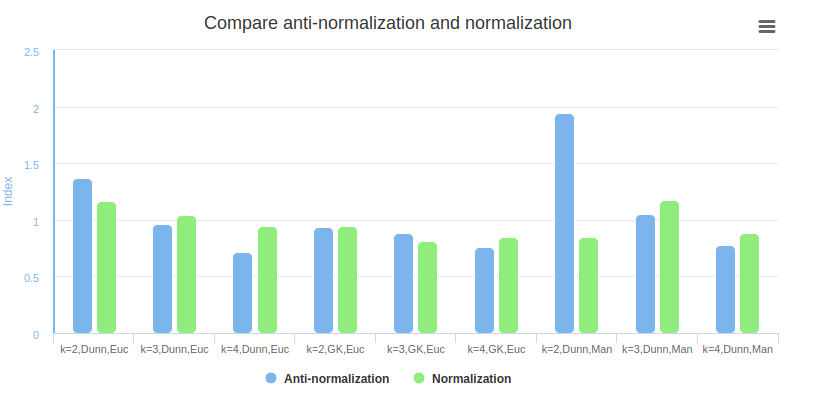
\includegraphics[width=\linewidth]{compare1.png}

\end{document}